\chapter{Using Plugins}\index{plugins}
\section{An Introduction to Using Plugins}
QGIS has been designed with a plugin architecture. This allows new features/functions to be added to the application. Many of the features in QGIS are actually implemented as plugins.

There are two types of plugins in QGIS: core and user-contributed.
\index{plugins!types}A core plugin is maintained by the QGIS development team and is part of every QGIS distribtution. A user-contributed plugin is an external plugin that is maintained by the individual author. The QGIS Community site (\url{http://community.qgis.org}) serves as the repository for user contributed plugins.

\subsection{Finding and Installing a Plugin}
When you install QGIS, all of the core plugins are included (these are described
below). \index{plugins!installing}Additional user-contributed plugins may be
available on the QGIS Community site. To see what user-contributed plugins are
available, see the plugins page on the Community site
(\url{http://community.qgis.org/plugins}).\index{plugins!user contributed}

Typically user-contributed plugins are distributed in source form and require compiling. For instructions on building and installing a user-contributed plugin, see the documentation included with the plugin.
\subsection{Managing Plugins}\label{sec:managing_plugins}\index{plugins!managing}
Managing plugins consists of loading or unloading them from QGIS. Loaded plugins are "remembered" when you exit the application and restored the next time you run QGIS.

To manage plugins, open the \textsl{Plugin Manager} from the \textsl{Tools}
menu. \index{plugins!manager}The Plugin Manager displays all the available plugins and their status (loaded or unloaded). Figure \ref{fig:pluginmanager} shows the Plugin Manager dialog.

\begin{figure}[h]
   \begin{center}
   \caption{Plugin Manager}\label{fig:pluginmanager}\smallskip
   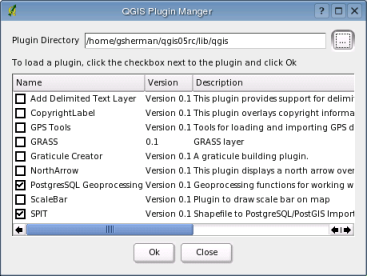
\includegraphics{qgis_user_guide_images/pluginmanager_80pct}
\end{center}  
\end{figure}
Typically all QGIS plugins are installed in the same location. This location is shown in the Plugin Directory text field. You can tell QGIS to load plugins from another location by specifying a different directory.
\begin{Tip}\caption{\textsc{Crashing Plugins}}\index{crashes}
\qgistip{If you find that QGIS crashes on startup, a plugin may be at fault. You can stop all plugins from loading by editing your .qt/qgisrc file in your home directory on Linux/Unix (Windows users will have to edit the registry). On Linux/Unix, open the qgisrc file in a text editor and find the [Plugins] section. Set all the plugin values to false to prevent them from loading. For example, to prevent the Delimited text plugin from loading, the entry in qgisrc should look like this:\ttfamily{
 Add Delimited Text Layer=false}.\normalfont  Do this for each plugin in the [Plugins] section. You can then start QGIS and add the plugins one at a time from the Plugin Manger to determine which is causing the problem.

}
\end{Tip} 

\subsection{Data Providers}\index{data providers}
Data Providers are "special" plugins that provides access to a data store. By default, QGIS supports PostGIS layers and disk-based data stores supported by the OGR library (Appendix \ref{appdx_ogr}). A Data Provider plugin extends the ability of QGIS to use other data sources.

Data Provider plugins are registered automatically by QGIS at startup. They are not managed by the Plugin Manager but are used behind the scenes when a corresponding data type is added as a layer in QGIS.
\subsection{Core Plugins}\index{plugins!core}
QGIS currently contains 9 core plugins that can be loaded using the Plugin Manager. Table \ref{tab:core_plugins} lists each of the core plugins along with a description of their purpose. Figure \ref{fig:plugintoolbar} shows the icon for each plugin in the Plugin toolbar (the number corresponds to the Item in Table \ref{tab:core_plugins}. Note the GRASS plugin is not included below because it installs its own toolbar (see Section \ref{sec:grass} for a discussion of available features in GRASS plugin).
\begin{table}[h]
\centering
\caption{QGIS Core Plugins}\label{tab:core_plugins}\medskip
\small
 \begin{tabular}{|l|l|p{4in}|}
\hline \textbf{Item} & \textbf{Plugin} & \textbf{Description} \\
\hline 1 & Copyright Label \index{plugins!copyright}& Display a copyright label on the map canvas\\
\hline 2 & Delimited Text \index{plugins!delimited text}& Load a delimited text file containing x,y coordinates as a point layer \\
\hline 3 & GPS Tools \index{plugins!gps}& Load and display GPS data \\
\hline 4 & Graticule Creator \index{plugins!graticule}& Create a latitude/longitude grid and save as a shapefile\\
\hline 5 & Scalebar \index{plugins!scalebar}& Add a scalebar to the map canvas\\
\hline 6 & North Arrow \index{plugins!north arrow}& Add a north arrow to the map canvas\\
\hline 7 & PostgreSQL Geoprocessing \index{plugins!geoprocessing}& Buffer a PostGIS layer \\
\hline 8 & SPIT \index{plugins!SPIT}& Shapefile to PostGIS Import Tool - import shapefiles into PostgreSQL\\
\hline
\end{tabular}
\end{table}
\normalsize
\begin{figure}[h]
   \begin{center}
   \caption{Plugin Toolbar and Icons}\label{fig:plugintoolbar}\smallskip
   
\includegraphics[scale=1.0]{qgis_user_guide_images/plugintoolbar}
\end{center}  
\end{figure}

\begin{Tip}\caption{\textsc{Plugins Settings Saved to Project}}\index{plugins settings}
\qgistip{When you save a .qgs project, any changes you have made to NorthArrow, ScaleBar and Copyright plugins will be saved in the project and restored next time you load it.
}
\end{Tip}
